\iffalse
\let\negmedspace\undefined
\let\negthickspace\undefined
\documentclass[journal,12pt,onecolumn]{IEEEtran}
\usepackage{cite}
\usepackage{amsmath,amssymb,amsfonts,amsthm}

\usepackage{graphicx}
\usepackage{textcomp}
\usepackage{xcolor}
\usepackage{txfonts}
\usepackage{listings}
\usepackage{enumitem}
\usepackage{mathtools}
\usepackage{gensymb}
\usepackage[breaklinks=true]{hyperref}
\usepackage{tkz-euclide} % loads  TikZ and tkz-base
\usepackage{listings}
\usepackage{gvv}
\usepackage{booktabs}

%
%\usepackage{setspace}
%\usepackage{gensymb}
%\doublespacing
%\singlespacing

%\usepackage{graphicx}
%\usepackage{amssymb}
%\usepackage{relsize}
%\usepackage[cmex10]{amsmath}
%\usepackage{amsthm}
%\interdisplaylinepenalty=2500
%\savesymbol{iint}
%\usepackage{txfonts}
%\restoresymbol{TXF}{iint}
%\usepackage{wasysym}
%\usepackage{amsthm}
%\usepackage{iithtlc}
%\usepackage{mathrsfs}
%\usepackage{txfonts}
%\usepackage{stfloats}
%\usepackage{bm}
%\usepackage{cite}
%\usepackage{cases}
%\usepackage{subfig}
%\usepackage{xtab}
%\usepackage{longtable}
%\usepackage{multirow}

%\usepackage{algpseudocode}
%\usepackage{enumitem}
%\usepackage{mathtools}
%\usepackage{tikz}
%\usepackage{circuitikz}
%\usepackage{verbatim}
%\usepackage{tfrupee}
%\usepackage{stmaryrd}
%\usetkzobj{all}
%    \usepackage{color}                                            %%
%    \usepackage{array}                                            %%
%    \usepackage{longtable}                                        %%
%    \usepackage{calc}                                             %%
%    \usepackage{multirow}                                         %%
%    \usepackage{hhline}                                           %%
%    \usepackage{ifthen}                                           %%
  %optionally (for landscape tables embedded in another document): %%
%    \usepackage{lscape}     
%\usepackage{multicol}
%\usepackage{chngcntr}
%\usepackage{enumerate}

%\usepackage{wasysym}
%\documentclass[conference]{IEEEtran}
%\IEEEoverridecommandlockouts
% The preceding line is only needed to identify funding in the first footnote. If that is unneeded, please comment it out.

\newtheorem{theorem}{Theorem}[section]
\newtheorem{problem}{Problem}
\newtheorem{proposition}{Proposition}[section]
\newtheorem{lemma}{Lemma}[section]
\newtheorem{corollary}[theorem]{Corollary}
\newtheorem{example}{Example}[section]
\newtheorem{definition}[problem]{Definition}
%\newtheorem{thm}{Theorem}[section] 
%\newtheorem{defn}[thm]{Definition}
%\newtheorem{algorithm}{Algorithm}[section]
%\newtheorem{cor}{Corollary}
\newcommand{\BEQA}{\begin{eqnarray}}
\newcommand{\EEQA}{\end{eqnarray}}
\newcommand{\define}{\stackrel{\triangle}{=}}
\theoremstyle{remark}
\newtheorem{rem}{Remark}

%\bibliographystyle{ieeetr}
\begin{document}
%

\bibliographystyle{IEEEtran}


\vspace{3cm}

\title{
%	\logo{
Gate 2021 Assignment 

\large{EE:1205 Signals and Systems}

Indian Institute of Technology, Hyderabad
%	}
}
\author{Abhey Garg

EE23BTECH11202
}	


% make the title area
\maketitle



%\tableofcontents


\renewcommand{\thefigure}{\theenumi}
\renewcommand{\thetable}{\theenumi}
%\renewcommand{\theequation}{\theenumi}

\section{Question EC 13}
The block diagram of a feedback control system is shown in the figure .
\begin{center}
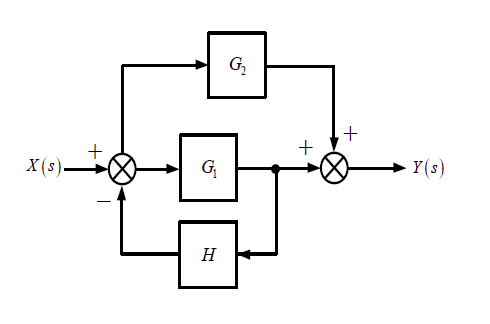
\includegraphics[width=0.5\textwidth]{2021/EC/13/figs/figure1.png}
\end{center}
The transfer function $\frac{Y(s)}{X(s)}$ of the system is :
\hfill(GATE 2021 EC)
\section{Solution}
\fi
\begin{table}[ht]
\centering
\setlength{\extrarowheight}{8pt}
\caption{Input Parameters}
\begin{tabular}{|c|l|l|} 
\hline
\textbf{Parameter} & \textbf{Used to denote} & \textbf{Values} \\
\hline
$n$ & Number of forward paths & \multicolumn{1}{|p{1.3cm}|}{\centering $2$ }\\
\hline
$\Delta_k$ & The value of $\Delta$ which is not touching the $k^{th} $ forward path & \multicolumn{1}{|p{1.3cm}|}{\centering $\Delta_1 = 1 , \Delta_2 = 1$ } \\
\hline
$\Delta$ & 1 - sum of the loop gains & \multicolumn{1}{|p{1.3cm}|}{\centering $1-G_1H$ } \\
\hline
$P_k$ & $k^{th}$ forward path gain & \multicolumn{1}{|p{1.3cm}|}{\centering $P_1 = G_1 , P_2 = G_2$ } \\
\hline
\end{tabular}
 \vspace{4mm}
\end{table}

According to Mason's gain formula , transfer function can be given as :
\begin{align}
\text{TF } &= \frac{\sum_{k-1}^{n} P_k \Delta_k}{\Delta} = \frac{P_1\Delta_1 + P_2\Delta_2}{\Delta} \\
&= \frac{G_1 + G_2 }{1 + G_1 H}
\end{align}
